\section{Data features and classic methods}
\label{sec:Data features and classic methods}
% 2 pages
To study the feasibility of this project, and to utilise deep learning methods to classify actions from sequential imagery features, videos containing pose-based data, comprehensively reviewing the previous research on data features and feature engineering methods is beneficial to the design of deep models.

%Characteristics of video-based data set
\begin{minipage}[ht]{.48\textwidth}
    \begin{figure}[H]
        \centering
        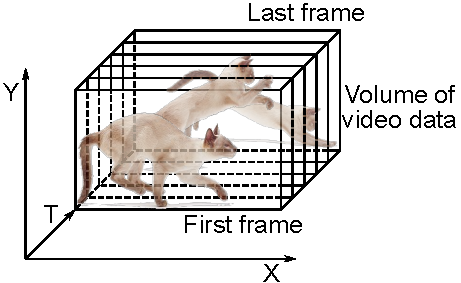
\includegraphics{literature/imgs/1-video-volume.pdf}
        \caption{Cubic volume of video data}
        \label{fig:1-video-volume}
    \end{figure}
\end{minipage}
\begin{minipage}[ht]{.5\textwidth}
    \begin{figure}[H]
        \centering
        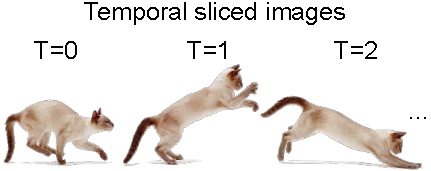
\includegraphics{literature/imgs/2-video-slice.pdf}
        \caption{Slicing the video cube parallel to the X-Y axis}
        \label{fig:2-video-slice}
    \end{figure}
\end{minipage}

Video is composed of a sequence of image data and synchronised audio arranged in the timeline. 
If the audio data beyond the scope of this study is ignored, the 2D images can be stacked along the time axis to form a 3D cube representing the video. Figure \ref{fig:1-video-volume} illustrates an intuitive representation proposed by \citet{fels1999interactive}, which highlights the spatial and temporal characteristics for all videos.
Further, figure \ref{fig:1-video-volume} shows that regular video frames produced by slicing the video cube parallel to the $X-Y$ axis so that computer vision algorithms or depth models for visual tasks can be applied.
As a result, video can be simplified into a series of images to enable applying image processing technology.

%Characteristics of human pose-based features
In each static image containing human pose-based features, what features can be used for posture analysis to classify each image? 
\citet{thrasher2011mood} model the features worthy of attention in human upper body posture and conduct pose-based study on mood recognition.

%Link pose-based and video-based features
From posture analysis in single imagery to human activity recognition in sequential imagery, it combines pose-based features and video-based data.
For example, \citet{yao2016spatio} propose a paper on spatio-temporal feature extraction with a variety of application scenarios in automatic human activity recognition, such as video information retrieval, intelligent surveillance, and human-computer interaction.
In future research, they will enable the low-level engineered features to fuse with a deep learning framework.

\citet{schuldt2004recognizing}

\citet{gorelick2007actions}

\citet{marszalek2009actions}

\citet{Soomro2014}